\documentclass[letterpaper, 12pt]{article}

\usepackage[utf8]{inputenc}
\usepackage[english, spanish]{babel}
\usepackage{fullpage}
\usepackage{graphicx}
\usepackage{amsmath}
\usepackage{enumitem}
\usepackage{chngcntr}
\usepackage{setspace}
\usepackage{url}
\usepackage{multicol}
\usepackage{csquotes}
\usepackage{float}
\usepackage{verbatim}
\usepackage{tabularx}
\usepackage{amsmath}
\usepackage{caption}
\usepackage{bm}
% \usepackage{hyperref}

\counterwithin{figure}{section}
\renewcommand{\thesection}{\arabic{section}}
\renewcommand{\thesubsection}{\thesection.\arabic{subsection}}
\renewcommand{\baselinestretch}{1.5}
\renewcommand{\thefigure}{\arabic{figure}}

\usepackage[style=numeric, maxnames=6, minnames=3, backend=biber, parentracker=true, sorting=none]{biblatex}
\DefineBibliographyStrings{english}{%chktex-file 1 chktex-file 6
	andothers = {\em et\addabbrvspace al\adddot}
}
\addbibresource{./Bibliography/bibliography.bib}

\usepackage{array}
\usepackage{enumitem}

\setlength{\parskip}{20pt}

\newcommand{\bolditalic}[1]{\textbf{\textit{#1}}}

% chktex-file 24

\begin{document}

\begin{titlepage}
	\centering
	\begin{multicols}{2}
		\begin{center}
			\begin{minipage}{0.4\textwidth}
				\centering
				
\includegraphics[width=0.7\linewidth]{Images/logo_utb.png}
			\end{minipage}
			\begin{minipage}{0.4\textwidth}
				\centering
				
\includegraphics[width=0.3\linewidth]{Images/png-transparent-js-react-js-logo-react-react-native-logos-icon-thumbnail.png}
			\end{minipage}
		\end{center}
	\end{multicols}

	{\scshape\LARGE Universidad Tecnológica de Bolívar \par}
	\vspace{1cm}

	{\scshape\Large FÍSICA CALOR Y ONDAS \par}
	\vspace{2.5cm}

	% chktex-file 8
	\slshape {\Large \bfseries{} Informe Final \\}
	\vspace{2cm}

	\slshape {\itshape{} Mauro González, T00067622 \\}
	\slshape {\itshape{} German De Armas Castaño, T00068765 \\}
	\slshape {\itshape{} Angel Vega Rodriguez, T00068186 \\}
	\slshape {\itshape{} Juan Jose Osorio Ariza, T00067316 \\}
	\slshape {\itshape{} Jorge Rueda Salgado, T00068722 \\}
	\vfill
	Revisado Por \\
	Yady Tatiana Solano Correa\\
	{\large \today\par}
\end{titlepage}

\nocite{source_code}
\nocite{vid_1}

% ! --------------------------------------------------------------------------------------------------------------------------------|>
\section*{\textit{Resumen}}

\begin{quote}
	A lo largo de la historia, las ondas sonoras han sido objeto de
	asombro y estudio. En nuestro proyecto ``Lectura de Ondas'',
	presentamos los resultados finales en los que hemos perfeccionado
	un programa capaz de recopilar y representar datos de audio en forma
	de ondas sonoras, resaltando sus propiedades clave. Nuestro enfoque
	en la tecnología del sonido se alinea con los Objetivos de Desarrollo
	Sostenible \textit{(ODS)} de las Naciones Unidas, particularmente en los campos
	de salud, educación e innovación. Este proyecto demuestra cómo la ciencia
	y la tecnología pueden contribuir al logro de un mundo más sostenible.
\end{quote}

% ! --------------------------------------------------------------------------------------------------------------------------------|>

\noindent\makebox[\linewidth]{\rule{\linewidth}{0.4pt}}

\bolditalic{Palabras claves}: \textit{Ondas sonoras, ondas electromiográficas,
	ingeniería del sonido, síntesis de sonido, espectro de
	onda.}

\noindent\makebox[\linewidth]{\rule{\linewidth}{0.4pt}}

% ! --------------------------------------------------------------------------------------------------------------------------------|>
\section*{Objetivos}

% + -------------------------------------------------------------------------|>
\subsection*{Objetivo general}

Diseñar una herramienta de lectura de ondas con el
propósito de adquirir, analizar y visualizar los datos
generados por ondas provenientes de distintas fuentes o
fenómenos, contribuyendo así a la comprensión y estudio de
sus características y patrones, que tenga el potencial de
evolucionar hacia una plataforma avanzada en el futuro.

% + -------------------------------------------------------------------------|>
\subsection*{Objetivos específicos}

\begin{itemize}[label=$\triangleright$]
	\item Perfeccionar la interfaz de usuario de nuestro programa,
	      siendo más intuitiva y permitiendo ofrecer una mejor
	      experiencia.

	\item Evaluar la estabilidad y funcionamiento del programa por
	      medio de extensas pruebas con distintos formatos de audio.
\end{itemize}

% + -------------------------------------------------------------------------|>
\subsection*{ODS Escogidas}

\begin{itemize}[label=$\triangleright$]
	\item (3) Salud y bienestar
	\item (4) Educación de calidad
	\item (9) Industria, innovación e infraestructura
\end{itemize}

¿POR QUÉ?

Nuestro proyecto ``Lectura de Ondas'' se adecúa a las ODS
3, 4 y 9 debido a su naturaleza multidisciplinaria y su
capacidad para abordar múltiples objetivos de desarrollo
sostenible.

La ODS 3 (Salud y Bienestar) encuentra relación en la
capacidad de nuestra herramienta para analizar ondas
sonoras al momento de aplicarse en un contexto urbano,
donde puede contribuir al monitoreó de frecuencias y
establecimiento de espacios neutros donde no se exponga la
integridad del oído humano.

La ODS 4 (Educación de Calidad) se ve respaldada por
nuestra herramienta al proporcionar recursos educativos
interactivos que mejoran la calidad de la educación al
permitir a estudiantes y docentes explorar conceptos de
física del sonido de manera práctica por medio de gráficas,
haciendo más fácil su comprensión y análisis.

La ODS 9 (Industria, innovación e infraestructura) debido a
que para analizar y comprender las ondas, el programa
utiliza tecnología avanzada (principalmente librerías para
el análisis de los MFCC o Mel Frequency Cepstral
Coefficients) que puede ser utilizada para diseñar
aplicaciones de reconocimiento de voz y hasta control por
voz (varias empresas han usado ecuaciones como la
transformada de Fourier para el reconocimiento de
tonalidades en la voz), lo cual es un claro ejemplo de
promoción de la innovación y el desarrollo tecnológico.

% ! --------------------------------------------------------------------------------------------------------------------------------|>
\section*{Marco Teorico}

% + -------------------------------------------------------------------------|>
\subsection*{Ondas~\cite{onda_definicion}}

Se conoce como onda a la propagación de energía (y no de
masa) en el espacio debido a la perturbación de alguna de
sus propiedades físicas, como son la densidad, presión,
campo eléctrico o campo magnético. Este fenómeno puede
darse en un espacio vacío o en uno que contenga materia, ya
sea agua, aire, tierra, etc.

% + -------------------------------------------------------------------------|>
\subsection*{Ondas sonoras~\cite{ondas_sonoras}}

Una onda sonora es una onda expansiva que puede ser
percibida por el oído humano. La onda sonora se puede
generar a partir del aparato fonador humano, mediante
máquinas, por animales, entre otras y se puede propagar en
distintos medios.

% + -------------------------------------------------------------------------|>
\subsection*{Amplitud~[A]}

Es la magnitud máxima del desplazamiento con respecto al
equilibrio, es decir, es la distancia existente entre la
posición de equilibrio y cualquiera de las posiciones
extremas. Su unidad de medidas en el Sistema Internacional
es el metro ($m$).

\begin{equation}
	A = \sqrt{x_{0}^{2} + \frac{v_{0x}^{2}}{\omega^{2}}}
\end{equation}

% + -------------------------------------------------------------------------|>
\subsection*{Periodo~[T]}

Es el tiempo que tarda una oscilación completa (ciclo), y
siempre es positivo. La unidad del periodo en el SI es el
segundo (s), aunque a veces se expresa como “segundos por
ciclo”.

% + -------------------------------------------------------------------------|>
\subsection*{Frecuencia~[f]}

Es el número de ciclos en la unidad de tiempo, y siempre es
positiva. La unidad de la frecuencia en el SI es el Hertz
($Hz$).

1 $Hz$ = 1 oscilación/segundo = $1s^{-1}$

% + -------------------------------------------------------------------------|>
\subsection*{Espectrómetro de sonido~\cite{espectometro}}

Es un dispositivo o programa informático que se utiliza
para visualizar y analizar las características espectrales
de una señal de audio. Básicamente, descompone una señal de
audio en sus componentes de frecuencia para proporcionar
información detallada sobre la distribución de energía en
diferentes bandas de frecuencia. Un espectrómetro de sonido
puede proporcionar información detallada sobre la amplitud
y frecuencia de los componentes de una señal de audio,
además, es importante destacar que tanto el hardware como
software pueden desempeñar el papel de un espectrómetro de
sonido. En el caso de software, librerías como ``librosa''
en Python pueden ser utilizadas para implementar
funcionalidades de espectro de sonido en aplicaciones de
procesamiento de audio.

% + -------------------------------------------------------------------------|>
\subsubsection*{Espectrograma~\cite{espectograma}}

El análisis espectral consiste en analizar una onda no
respecto a su forma de onda, sino respecto a las ondas
senoidales s que se deberían sumar para crear esa onda.
Este conjunto de ondas senoidales que es particular para
cada forma de onda especifica es lo que llamamos espectro
de frecuencia.

Un espectrograma es una representación visual de cómo varía
la energía de una señal de audio en función del tiempo y la
frecuencia. El espectro de una onda se obtiene atreves de
la ecuación llamada ``La transformada de Fourier''

\begin{equation}
	G(f) = \int_{-\infty}^{\infty } g(t) e^{-j 2 \pi f t} \,dx
\end{equation}

La lectura o comprensión del espectrómetro es la siguiente:

Eje horizontal (eje del tiempo): Generalmente de izquierda
a derecha. Cada punto en este eje corresponde a un momento
específico en la grabación de audio.

Eje vertical (eje de frecuencia): En esta parte de la
gráfica los componentes no se ven como líneas completamente
rectas, sino más bien como picos que sobresalen (por
errores de precisión del software). La proporción esta
demostrada en sus valores en decibeles, donde la onda de
menor frecuencia se le llama “fundamental” y el resto de
los múltiplos se les llaman “armónicos”. La fundamental es
la frecuencia de la onda entera y determina la nota musical
que predomina, mientras que los armónicos proporcionan la
forma de la onda y el timbre de esta. Las frecuencias más
bajas suelen estar en la parte inferior, mientras que las
frecuencias más altas están en la parte superior.

% + -------------------------------------------------------------------------|>
\subsection*{Intensidad del color o brillo}

Indica la amplitud o energía de cada frecuencia en un
momento específico. Los colores más oscuros o brillantes
indican una mayor energía en esa frecuencia en ese momento
particular.

% + -------------------------------------------------------------------------|>
\subsection*{Intensidad de sonido}

La intensidad de sonido se refiere a la cantidad de energía
que transporta una onda de sonido por unidad de área en una
dirección perpendicular al flujo de la onda.

En términos más simples, la intensidad de sonido representa
cuán fuerte o débil es una onda sonora en un punto
específico del espacio. La intensidad de sonido se mide en
vatios por metro cuadrado (W/m²) y puede variar ampliamente
en diferentes situaciones.

\begin{equation}
	I = \frac{\frac{E}{t}}{A} = \frac{P}{A}
\end{equation}

% + -------------------------------------------------------------------------|>
\subsection*{Decibeles}

Son una unidad de medida que se utiliza para expresar la
relación entre dos cantidades, generalmente en términos de
potencia, intensidad o nivel de presión.

\begin{equation}
	\beta = 10 \log \frac{I}{I_{0}}
\end{equation}

Donde, $I_{0}$ es $10^{-12} \frac{W}{m^{2}}$

% + -------------------------------------------------------------------------|>
\subsection*{MFCC~\cite{mfcc}}

Los Coeficientes Ceptrales en las Frecuencias de Mel (MFCC,
por sus siglas en inglés: Mel Frequency Cepstral
Coefficients) son una representación de las características
espectrales de una señal de audio, diseñada para imitar
ciertas características del sistema auditivo humano.

Para ser mas detallado los MFCC involucran:

\begin{enumerate}
	\item Mel Escala: La escala de Mel es una escala de frecuencia no
	      lineal que se basa en cómo percibimos las diferencias entre
	      tonos en diferentes partes del espectro de frecuencias. La
	      escala de Mel es más adecuada para representar la
	      percepción auditiva humana que la escala lineal de Hertz.

	\item Cepstrum: El cepstrum es la transformada inversa de la
	      transformada de Fourier de un logaritmo del espectro de
	      potencia. En términos sencillos, representa cómo cambian
	      las características en el dominio de la frecuencia en el
	      dominio cepstral (que es el logaritmo de la frecuencia).
	      Esto es útil para separar las características relevantes
	      del espectro de potencia.

	\item Coeficientes Cepstrales: Una vez que se ha calculado el
	      cepstrum, se selecciona un conjunto de coeficientes que
	      capturan las características más importantes de la señal.
	      Estos coeficientes representan cómo varía la energía en
	      diferentes bandas de frecuencia en la escala de Mel.

	      Los MFCC se utilizan comúnmente en aplicaciones de
	      procesamiento de voz y audio, como el reconocimiento
	      automático del habla, la síntesis de voz, la clasificación
	      de género, entre otras.
\end{enumerate}

% + -------------------------------------------------------------------------|>
\subsection*{Tonalidad en el sonido~\cite{tonalidad}}

La tonalidad en el contexto del sonido se refiere a la
percepción subjetiva de la altura o agudeza de un tono
musical. En otras palabras, la tonalidad nos dice si un
sonido se percibe como agudo o grave.

La tonalidad está directamente relacionada con la
frecuencia de una onda sonora. Frecuencias más altas
corresponden a tonos más agudos, mientras que frecuencias
más bajas corresponden a tonos más graves.

En el sistema musical occidental, la tonalidad se organiza
en una escala cromática compuesta por 12 tonos, cada uno
separado por un semitono. Cada tono tiene una frecuencia
específica asociada y está etiquetado con una nota musical
(por ejemplo, Do, Re, Mi, etc.)

% ! --------------------------------------------------------------------------------------------------------------------------------|>
\section*{Procedimiento experimental}

\begin{figure}[H]
	\begin{center}
		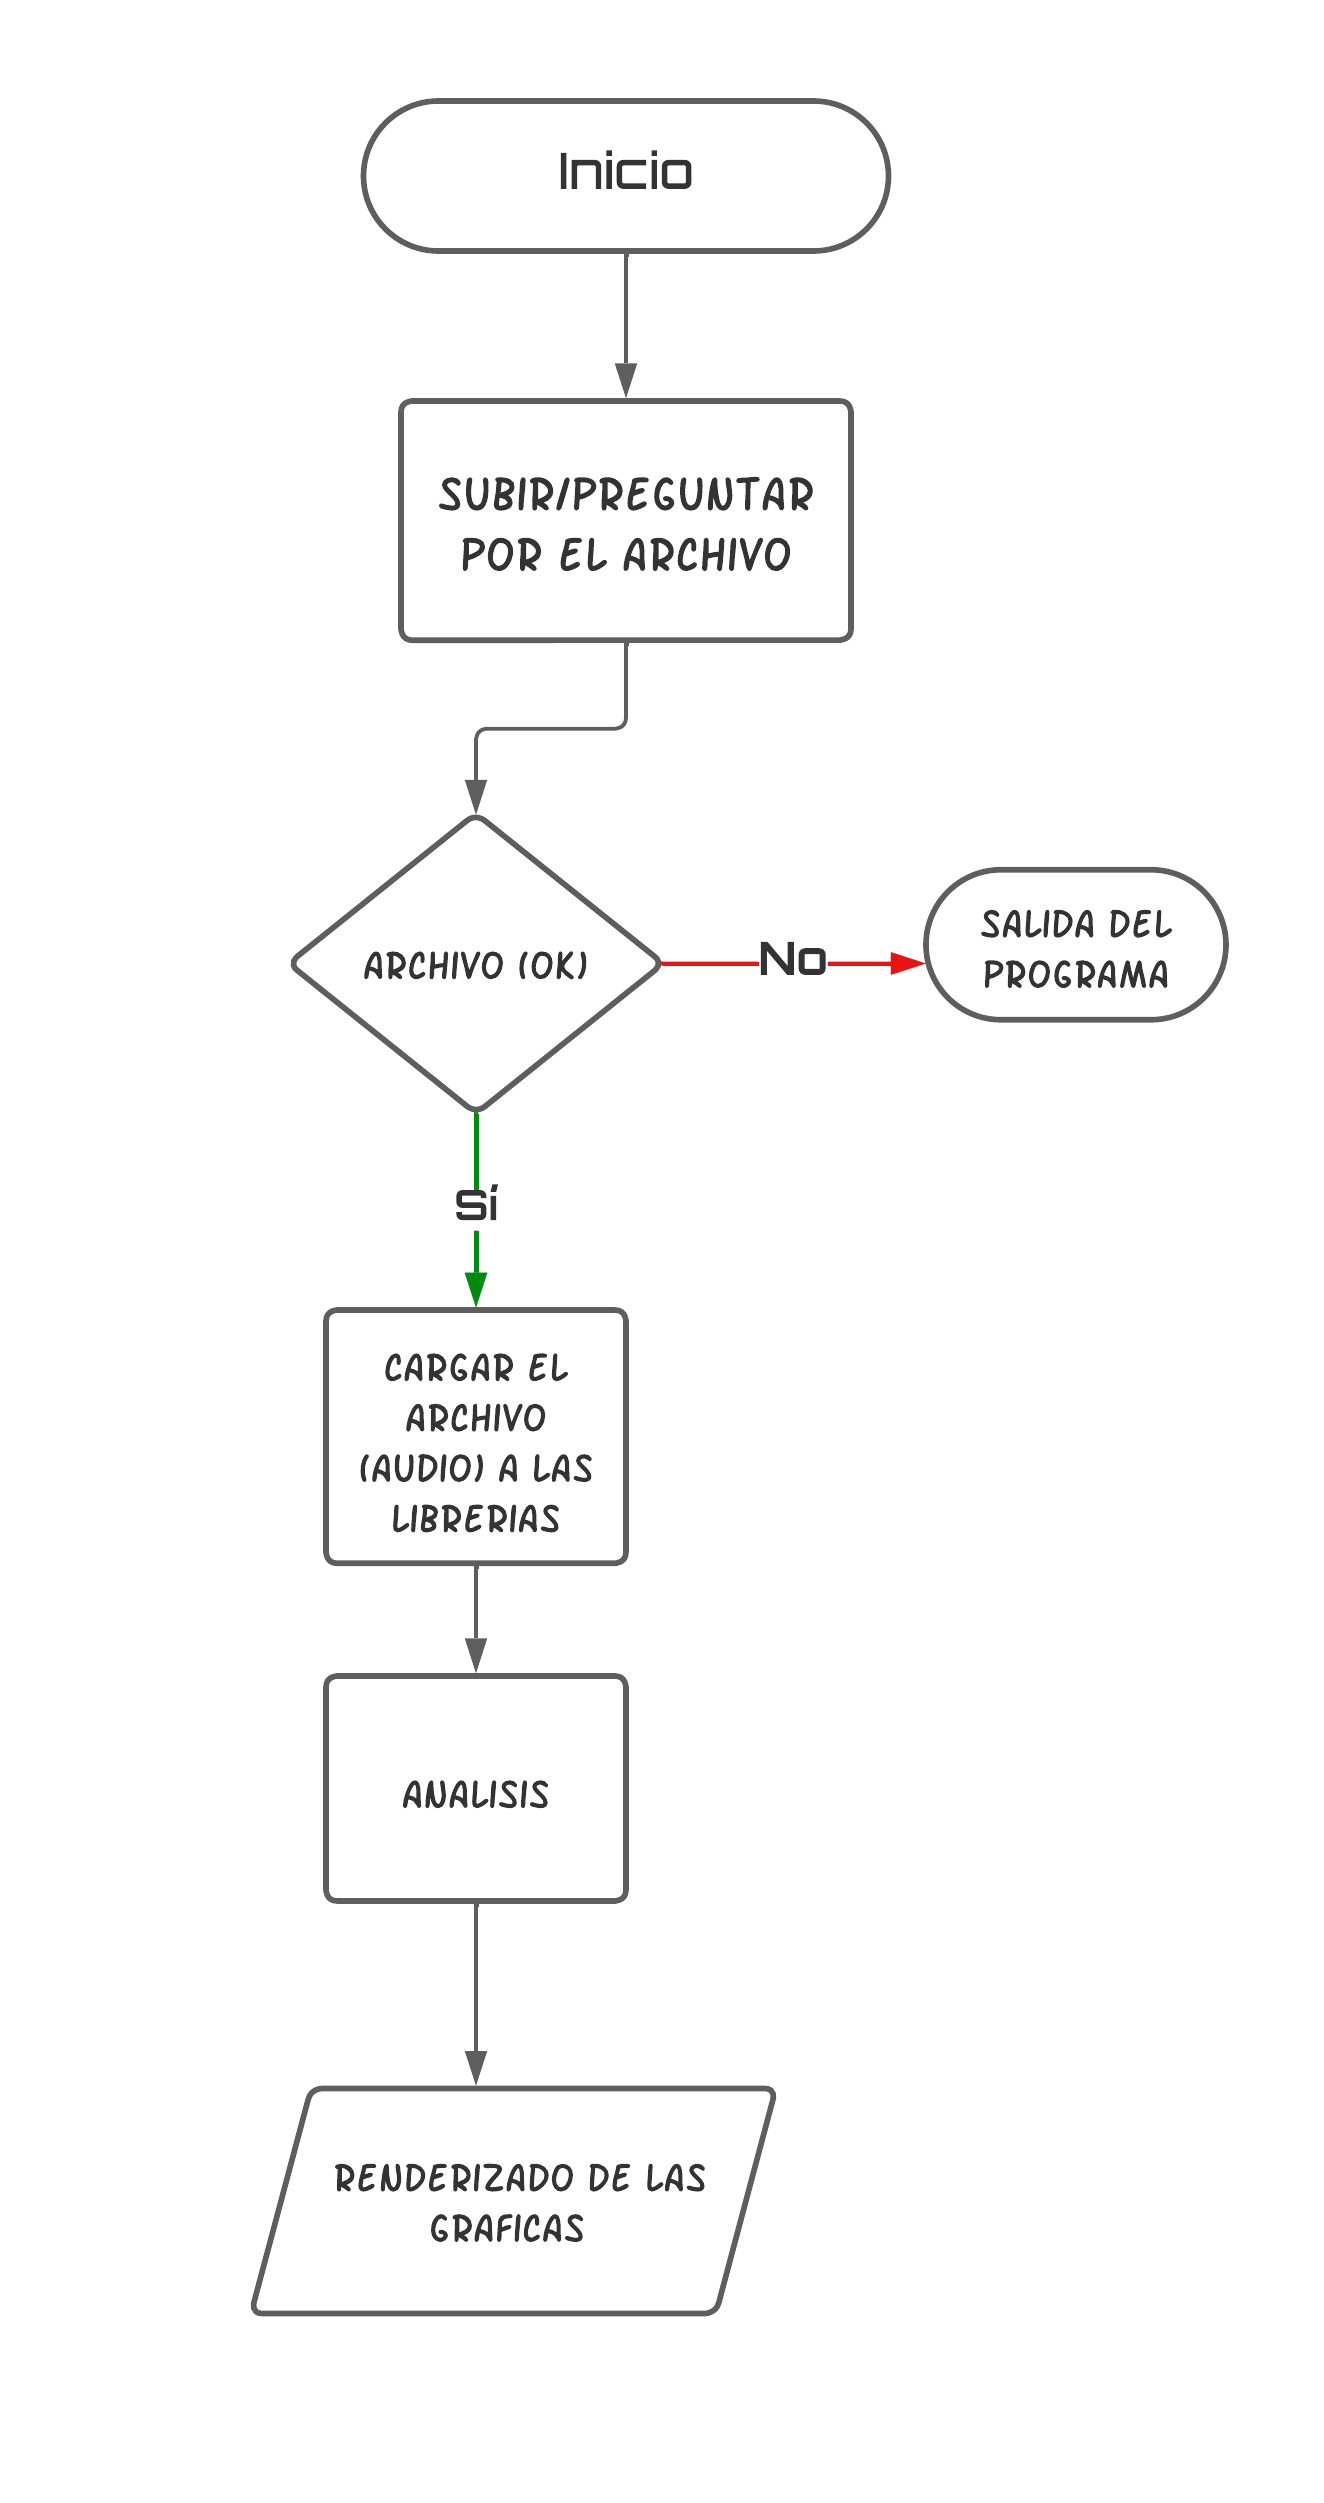
\includegraphics[width=.4\linewidth]{Images/Flujograma.png}
		\caption{}
	\end{center}
\end{figure}

Basado en el diagrama de flujo, asimismo son los pasos que
se llevaron a cabo en el programa. Cabe mencionar que la
aplicación esta escrita en \textit{React}

\begin{enumerate}
	\item Detección del audio y envió al servidor
	      \begin{figure}[H]
		      \begin{center}
			      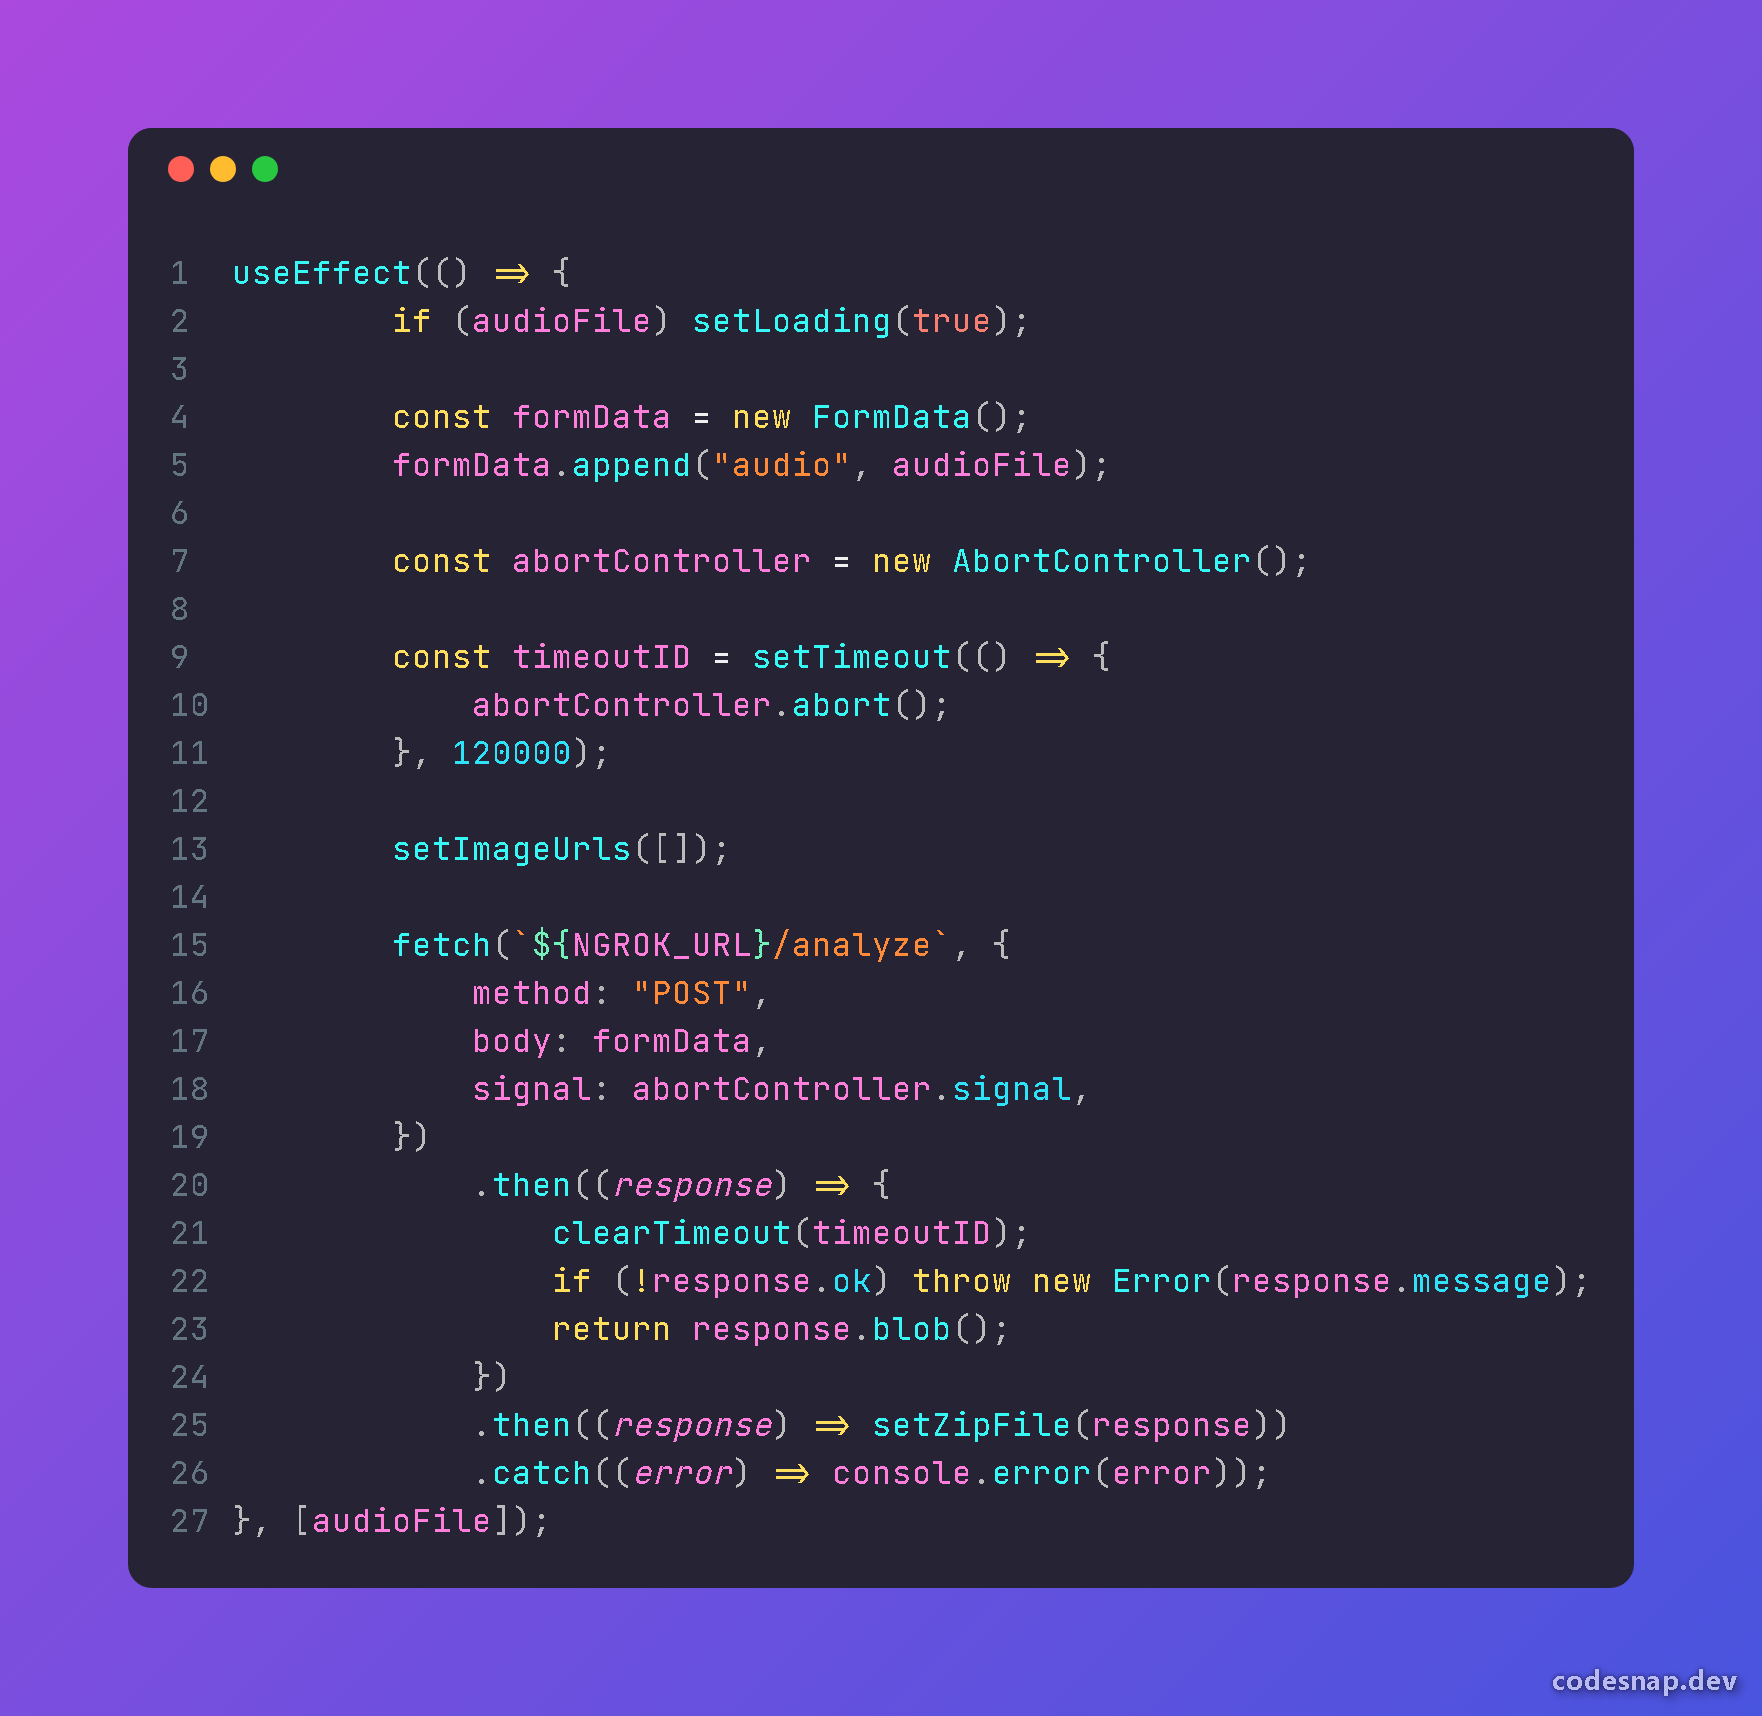
\includegraphics[width=.8\linewidth]{Images/UploadAudioFile.png}
		      \end{center}
	      \end{figure}

	      En este \textit{snippet} haciendo uso del
	      \textit{useEffect}, por parte de \textit{React} que se
	      encarga de detectar en cuanto haya un cambio en
	      \textit{audioFile} que seria el archivo de audio que
	      cargará el usuario.

	      Luego se agrega este mismo archivo de audio a un objeto
	      \textit{formData} para que pueda ser enviado en el
	      \textit{body} de una solicitud \textit{http}, ademas de
	      declarar un \textit{AbortController} para cancelar la misma
	      solicitud en caso de un \textit{timeout}.

	      Después de esto, se procede a realizar la solicitud
	      haciendo uso de la instrucción \textit{fetch}, agregando el
	      \textit{body} de la solicitud.

	      Por ultimo, dependiendo de la respuesta del servidor se
	      toman acciones, en caso de un \textit{success}, se procede
	      a renderizar las imágenes, mientras que en caso de un
	      \textit{error} se muestra por consola y se interrumpe la
	      ejecución.

	\item Recibir el análisis completo
	      \begin{figure}[H]
		      \begin{center}
			      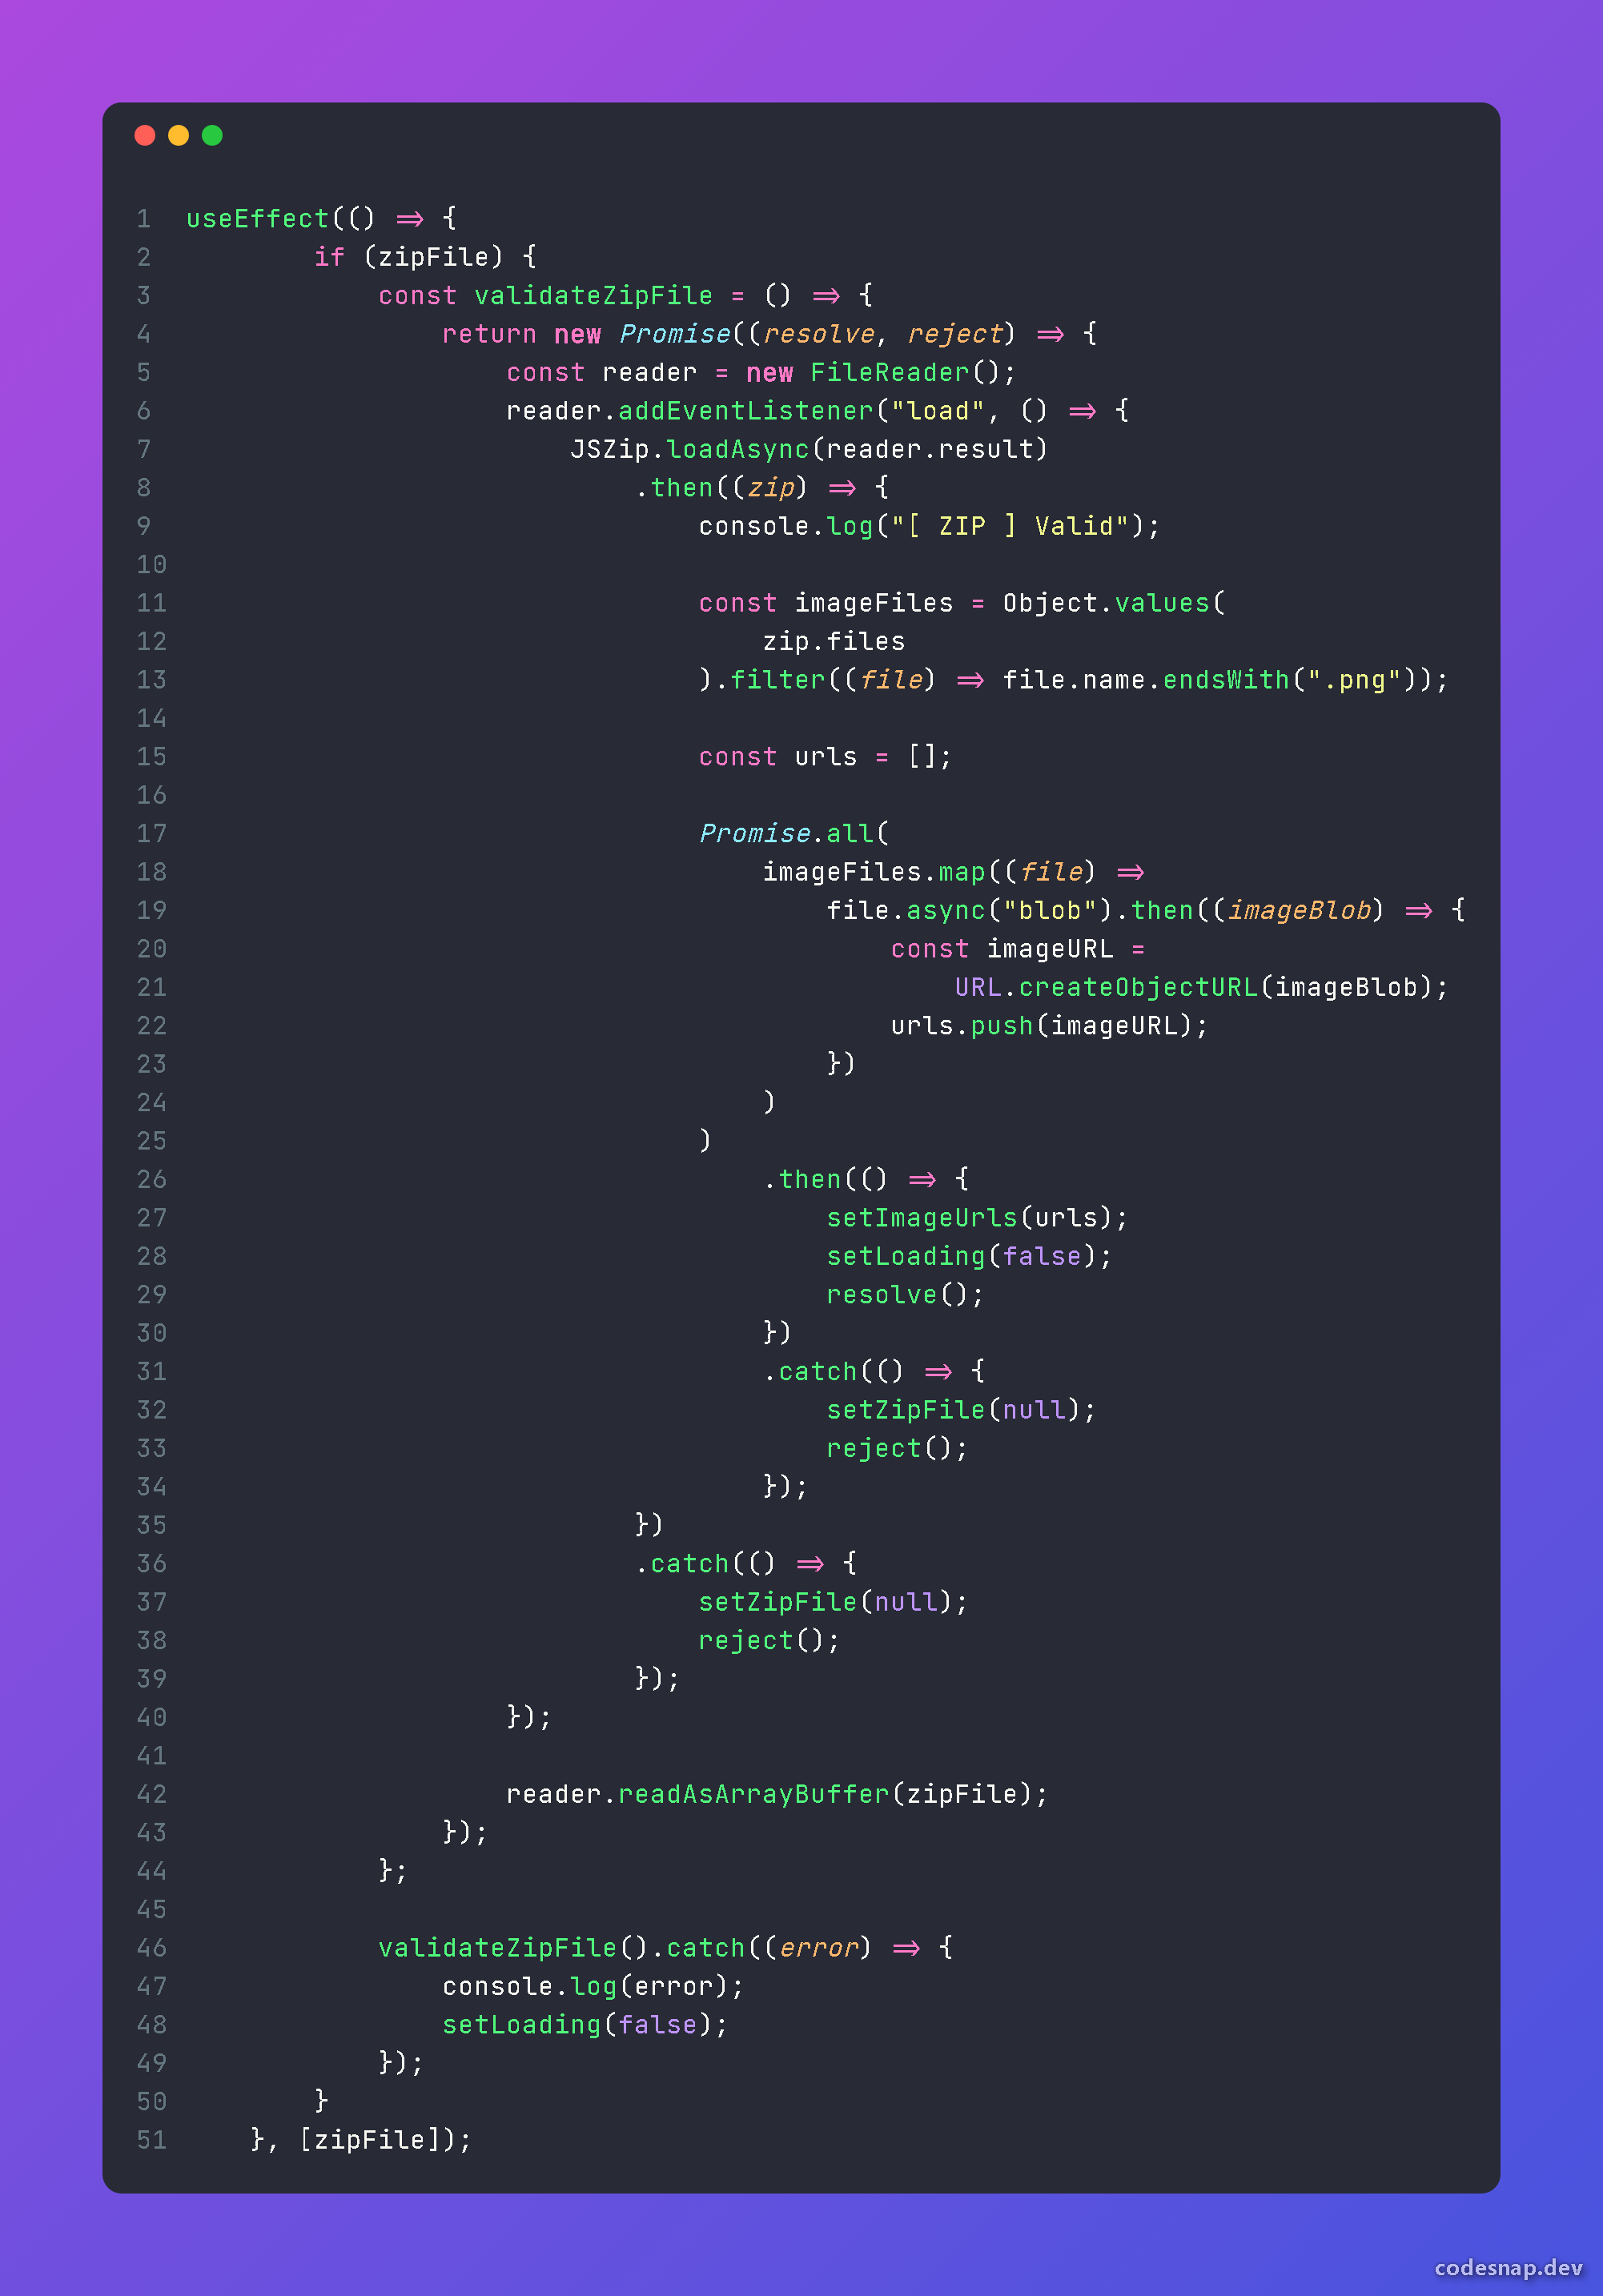
\includegraphics[width=.7\linewidth]{Images/SendAudioToAPI.png}
		      \end{center}
	      \end{figure}

	      Similarmente, luego de detectar un cambio en el archivo
	      \textit{zipFile}, se procede a descomprimirlo haciendo uso
	      de \textit{JSzip} (modulo), para ademas verificar en caso
	      de que tenga un error el archivo.

	\item Renderizado de las imágenes
	      \begin{figure}[H]
		      \begin{center}
			      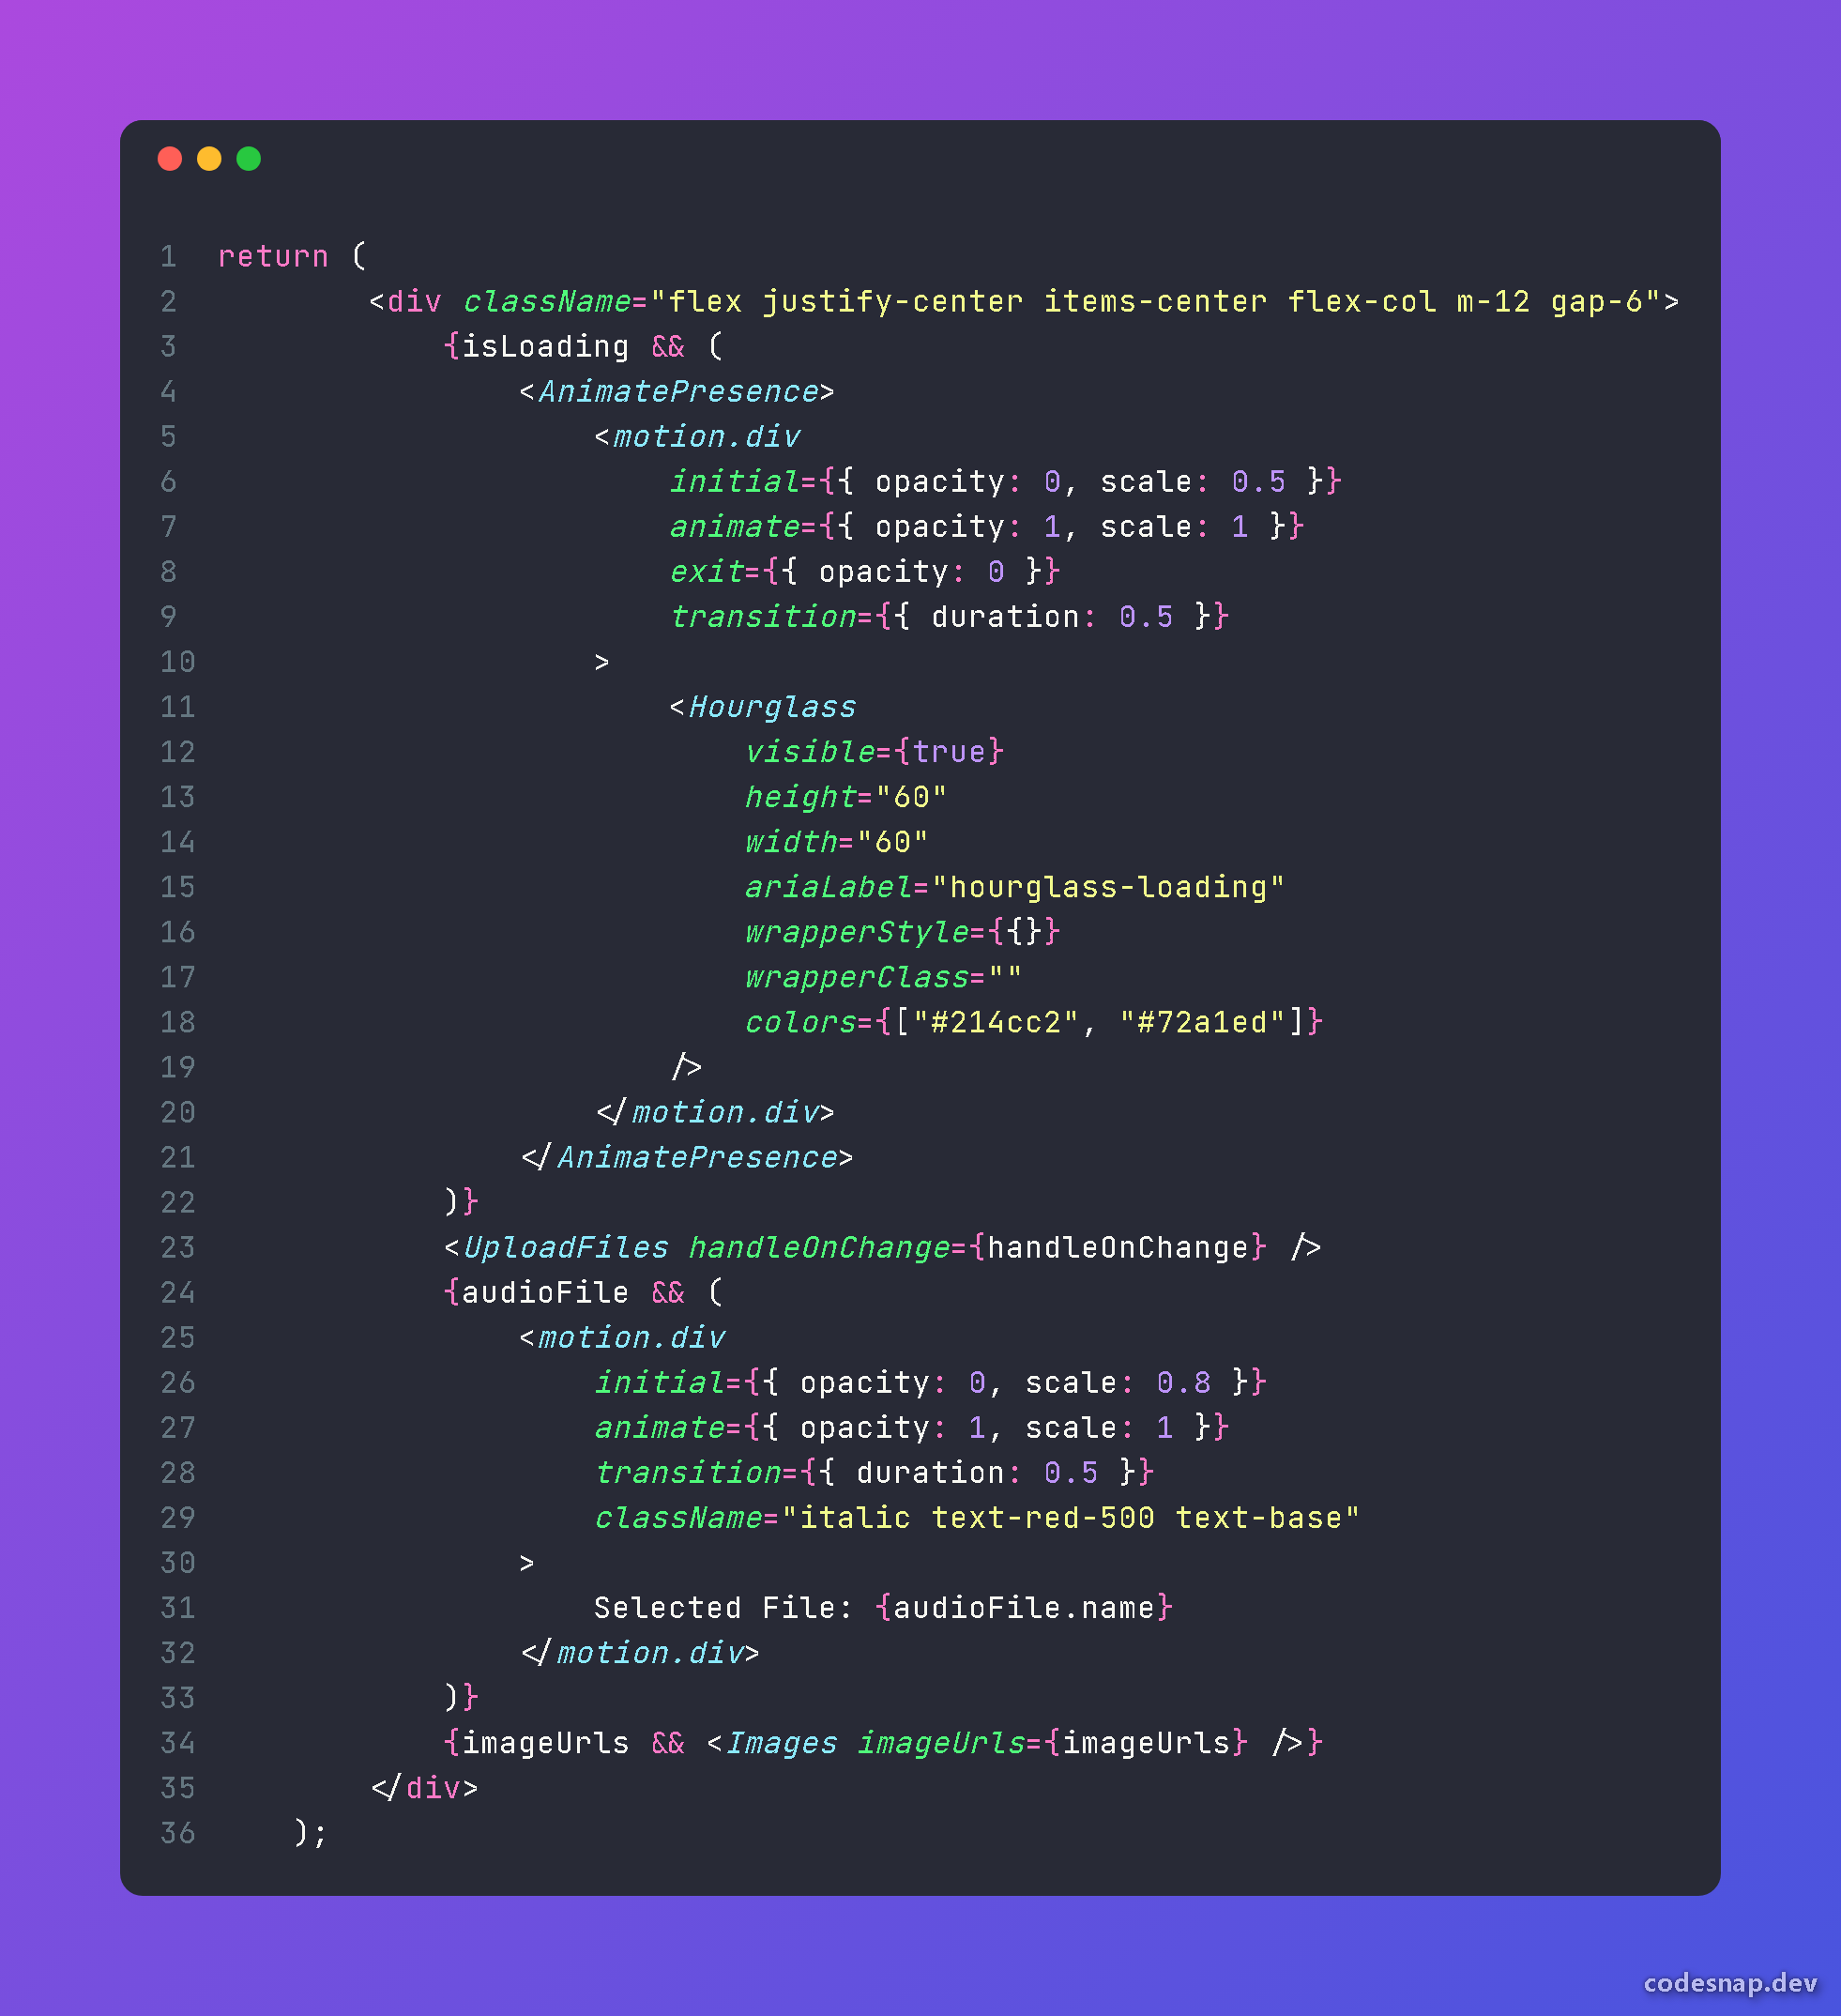
\includegraphics[width=.8\linewidth]{Images/RenderizeApp.png}
		      \end{center}
	      \end{figure}

	      Por ultimo, cuando se detecta un cambio de estado en el
	      \textit{array} que guarda las imágenes, proceden a ser
	      renderizadas en el \textit{UI}.
\end{enumerate}

% ! --------------------------------------------------------------------------------------------------------------------------------|>
\section*{Datos experimentales}

\nocite{ClownCore}

Para probar la app, se utilizo la canción \textit{``Song''}
de \textit{ClownCore} y estas fueron los resultados:

\begin{figure}[H]
	\begin{center}
		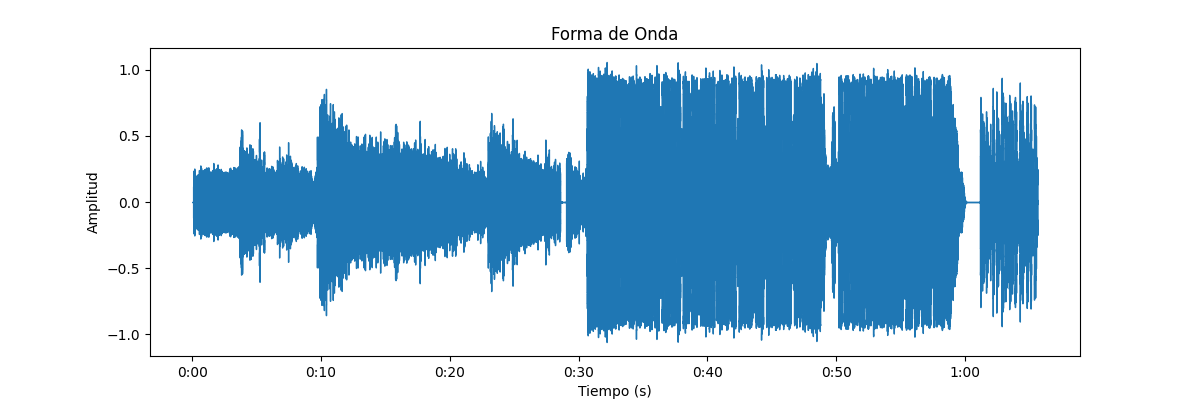
\includegraphics[width=\linewidth]{Images/testWaveShape.png}
		\caption{}
	\end{center}
\end{figure}

\begin{figure}[H]
	\begin{center}
		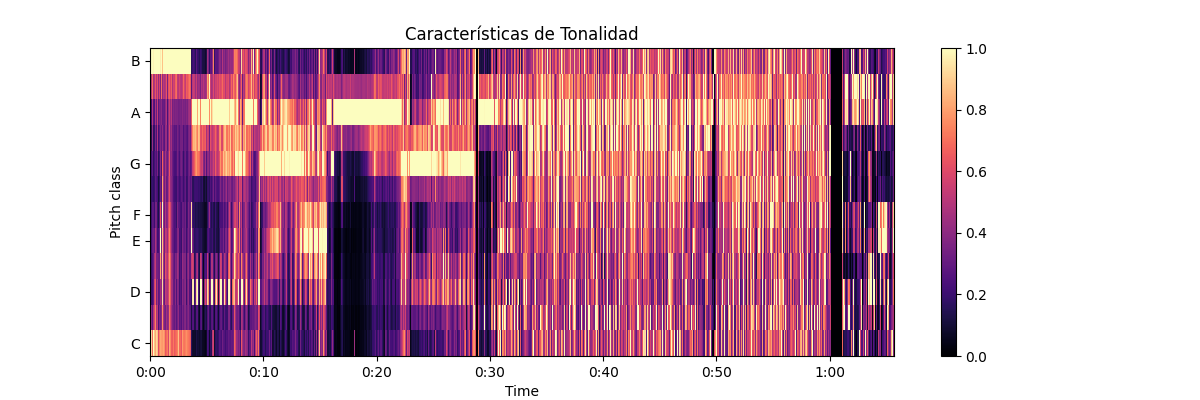
\includegraphics[width=\linewidth]{Images/testTonality.png}
		\caption{}
	\end{center}
\end{figure}

\begin{figure}[H]
	\begin{center}
		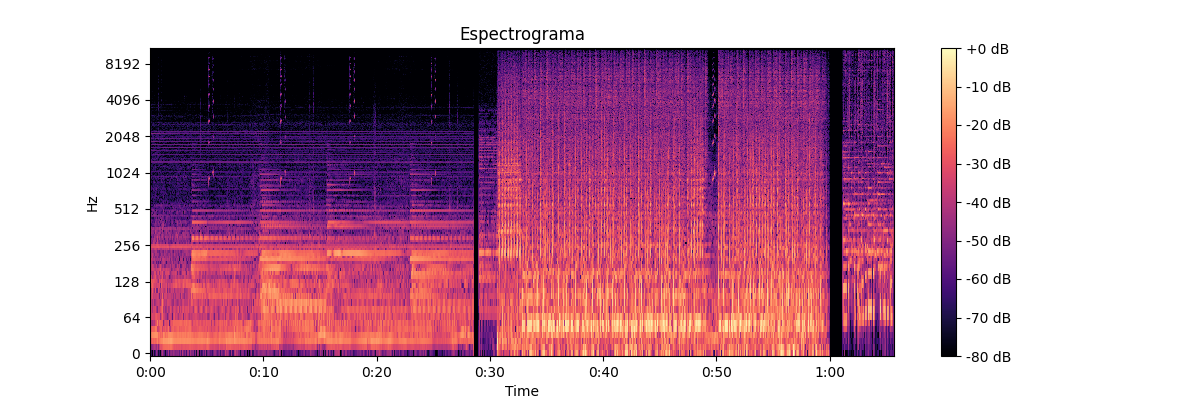
\includegraphics[width=\linewidth]{Images/testSpectogram.png}
		\caption{}
	\end{center}
\end{figure}

\begin{figure}[H]
	\begin{center}
		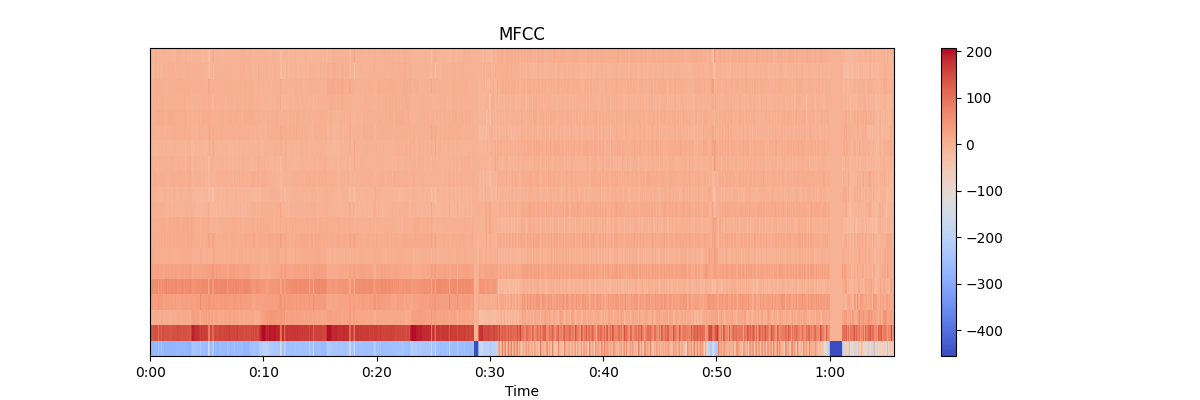
\includegraphics[width=\linewidth]{Images/testMFCC.png}
		\caption{}
	\end{center}
\end{figure}

% ! --------------------------------------------------------------------------------------------------------------------------------|>
\section*{Conclusiones}

Esta entrega muestra nuestro proyecto final, en el que los
logros conseguidos nos han permitido perfeccionar nuestra
herramienta, estableciendo finalmente de manera óptima el
filtrado de los datos mediante el programa, logrando
ofrecer una experiencia más intuitiva y llamativa
visualmente al usuario. Con esto en mente, abordamos la
salud y el bienestar a través del análisis de sonido,
mejorar la calidad de la educación al proporcionar recursos
educativos y promover la industria, la innovación y la
infraestructura a través de tecnología en el procesamiento
de ondas sonoras, logrando un enfoque multidisciplinario lo
que demuestra una gran capacidad y relevancia para cumplir
objetivos de desarrollo sostenible.

\nocite{source_code}

\printbibliography

\end{document}